\section{Time box 3}
\subsection{Time box planning}

\begin{figure}[H]
	\begin{centering}
		 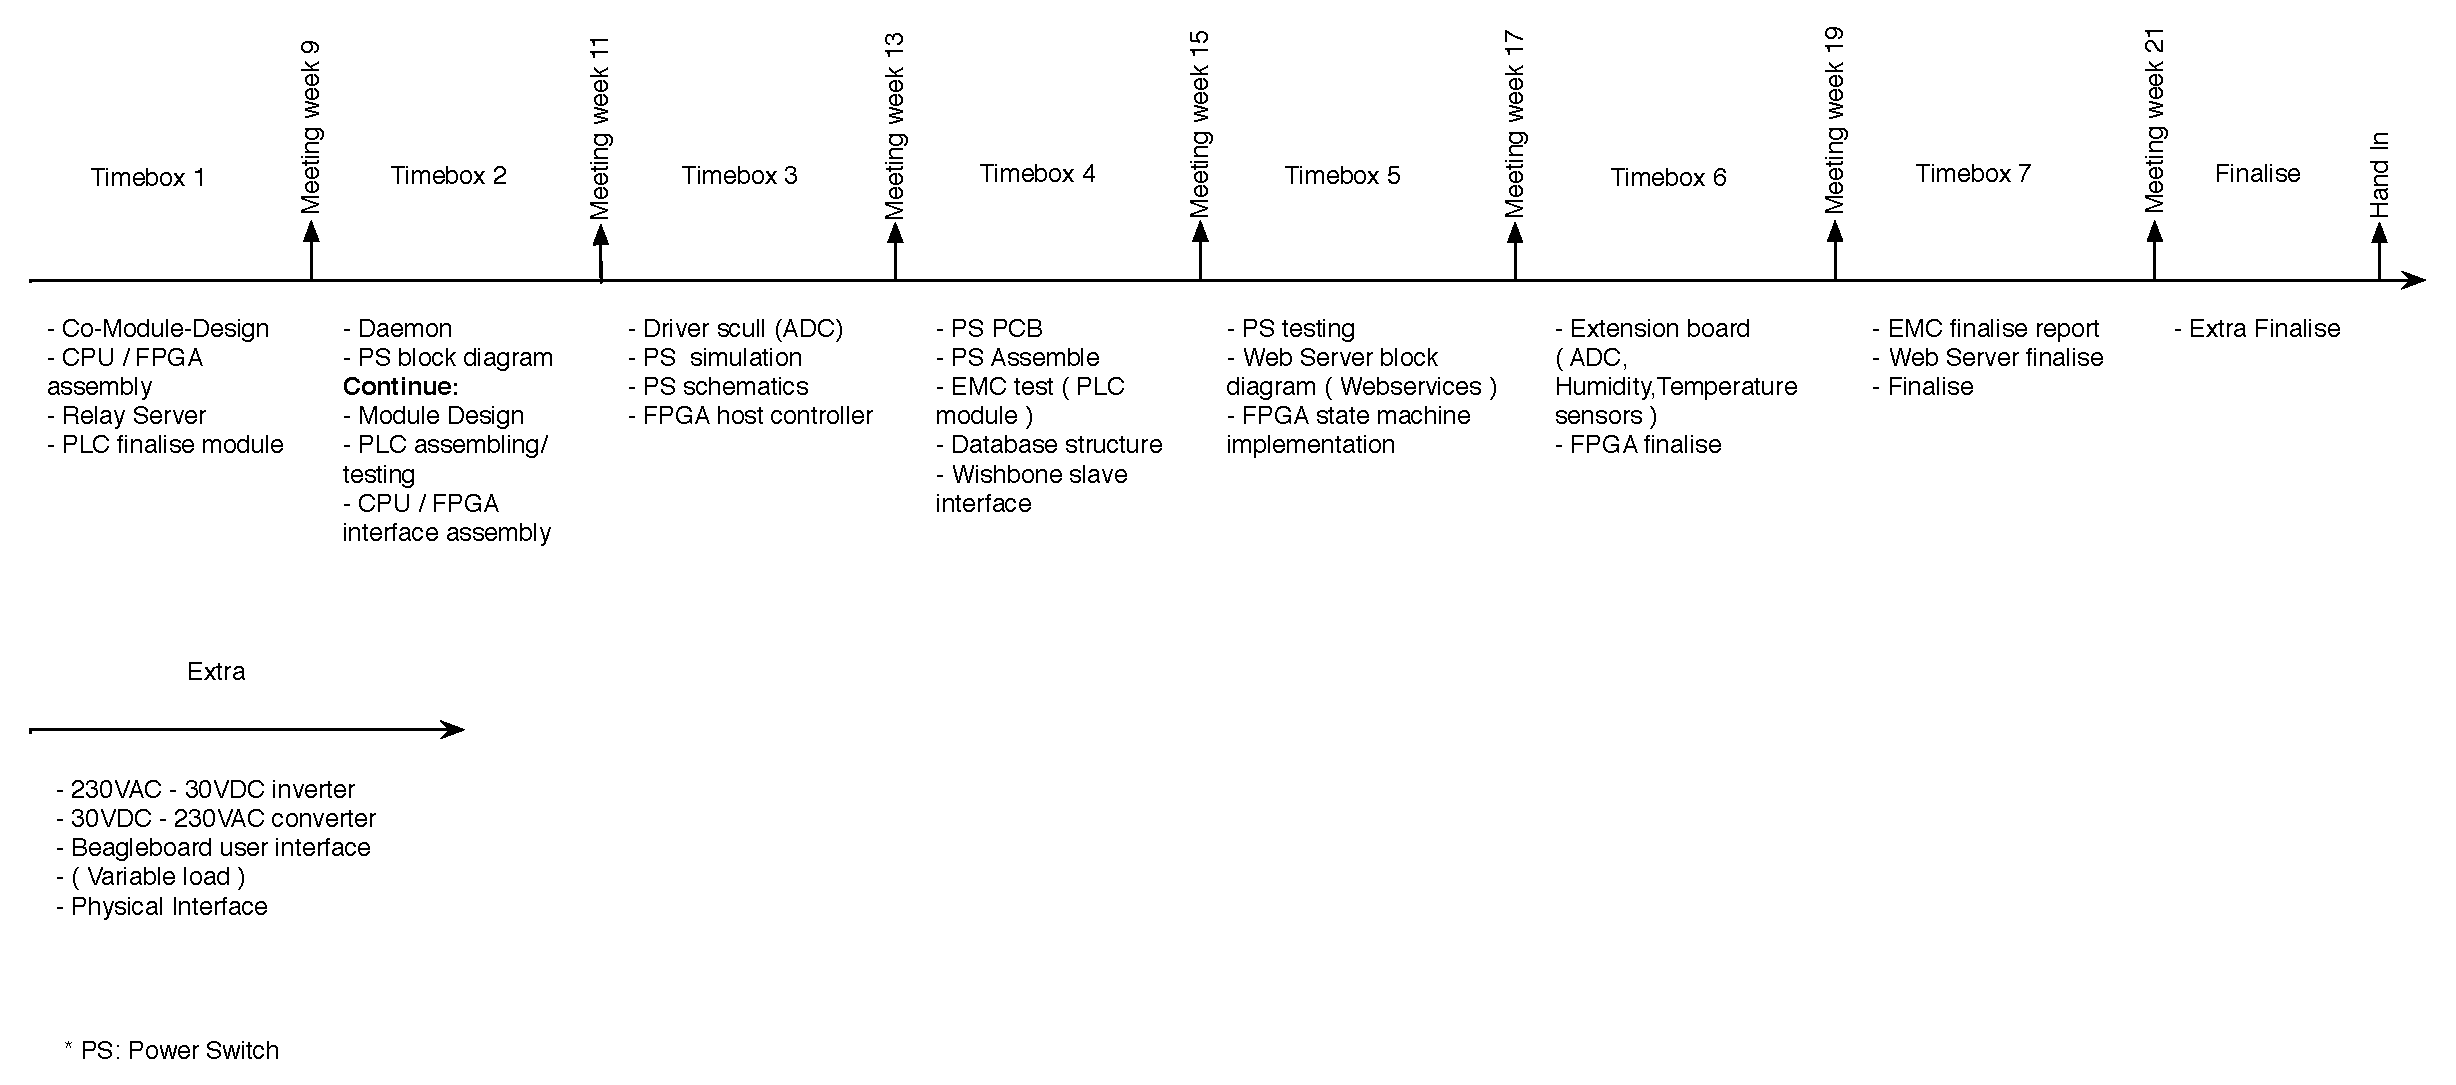
\includegraphics[width=1.0\textwidth]{images/tb_r3.pdf}
		\caption{Updated time-box}
	\end{centering}
\end{figure}

\subsubsection{Work to be done in this time box}
\begin{itemize}
	\item Device driver
	\begin{itemize}
		\item Create a device driver framework from the scull example and the device drivers included in the distribution. 
		\item Convert the ADC driver into a device driver.
	\end{itemize}
	\item Power switch
	\begin{itemize}
		\item Schematic
		\item Printed circuit board
		\item Mount component
		\item Power Switch Test
		\item Further Implementations
	\end{itemize}
	\item{Webserver Communication}
	\begin{itemize}
		\item Data Flow
		\item Setting the Server
		\item Further implementations
	\end{itemize}
	\item Host controller
	\begin{itemize}
		\item Master wishbone
		\item CPU interface
	\end{itemize}
\end{itemize}
\paragraph{Description:}
\begin{description}
	\item[Power switch] A single switch port board for the power switch is made, as an essential part for the power switch.
	\item[Host controller] is made in the FPGA, and is responsible for the communication between the Spartan6 and the ARM7, it shall be made with wishbone master interface 
\end{description}

\subsection{Power switch}
Power switch module have to be able to switch the power direction. A battery after fully charged can be used to power other modules or systems.

The power switch module have to be able to switch the power direction so for instance a battery fully charged can be used to power other modules or systems but also to protect the different modules connected to the hub.

\subsubsection{Schematics}

\begin{figure}[H]
	\begin{centering}
		 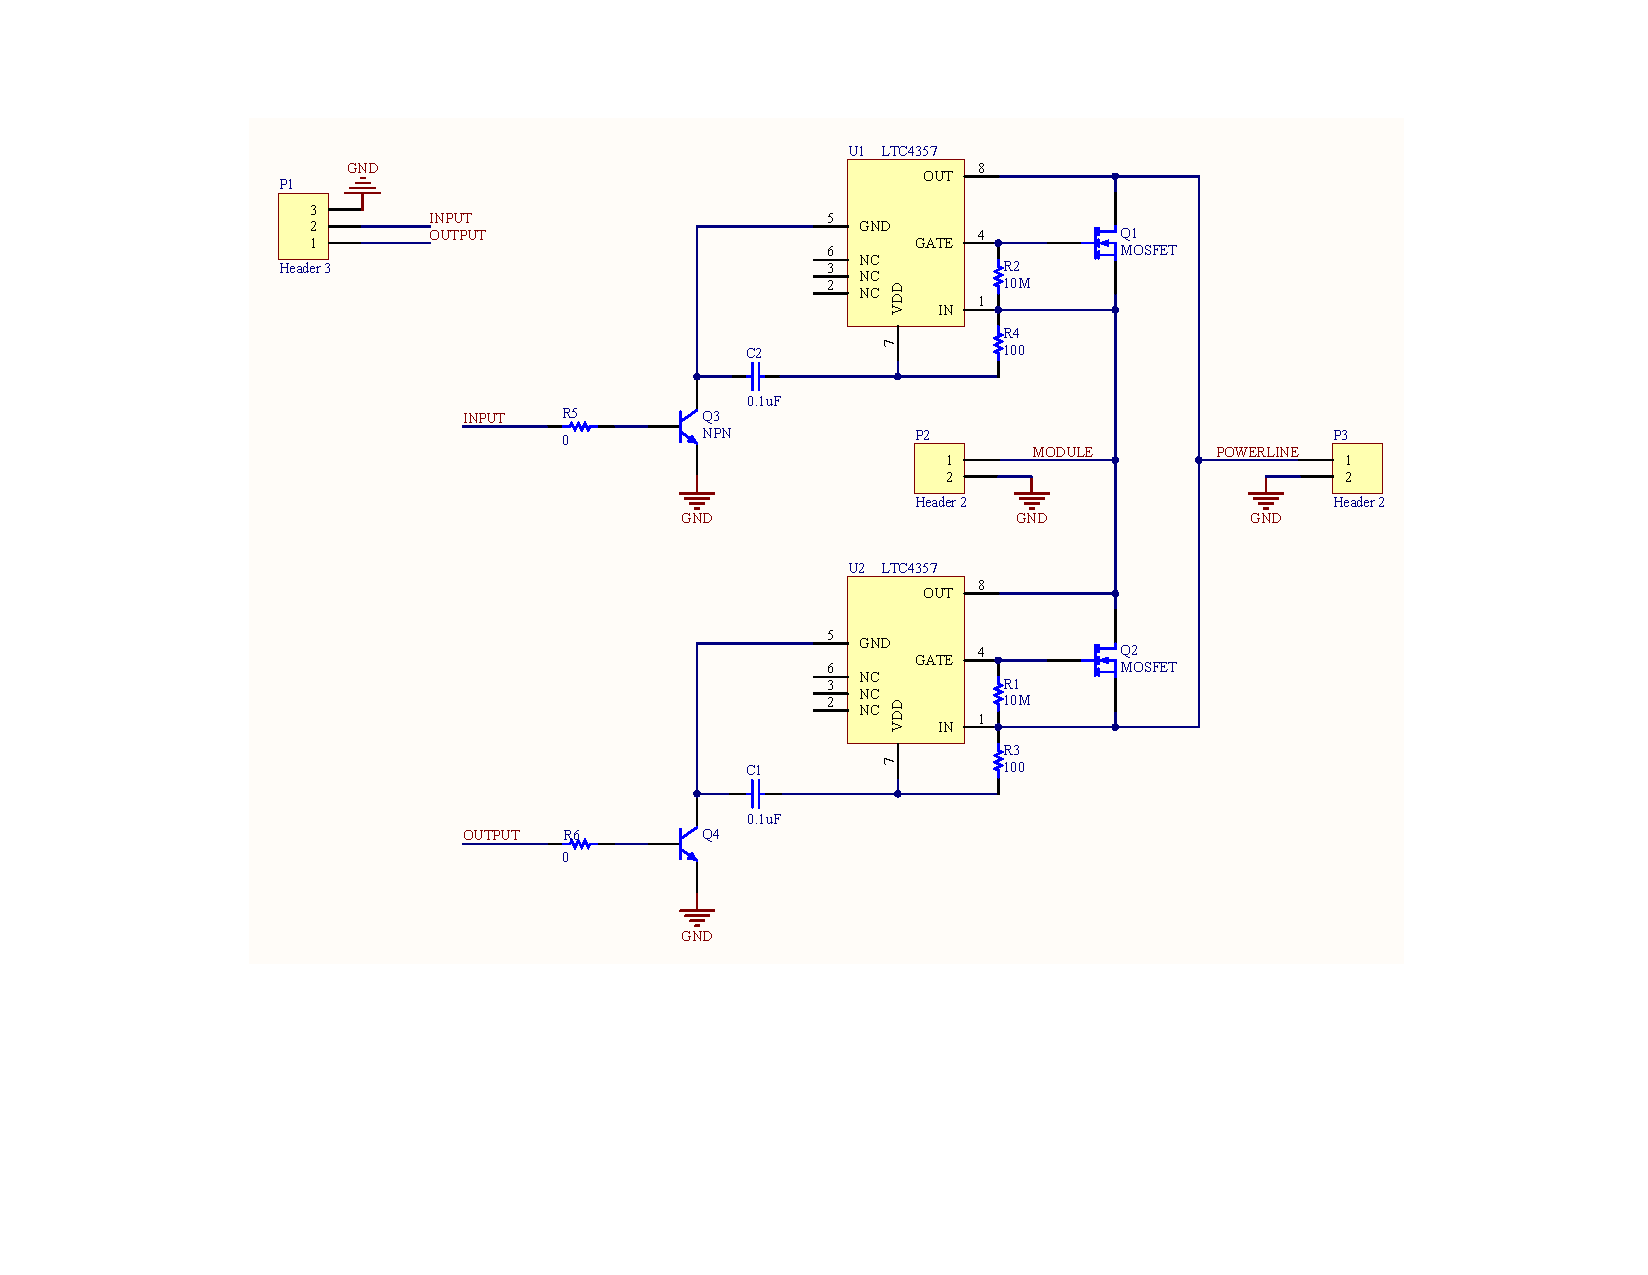
\includegraphics[width=1.0\textwidth,page=1]{images/ps_schematics.pdf}
		\caption{Schematic of the switch interface}
	\end{centering}
\end{figure}

\subsubsection{Printed circuit board}

\begin{figure}[H]
	\begin{centering}
		 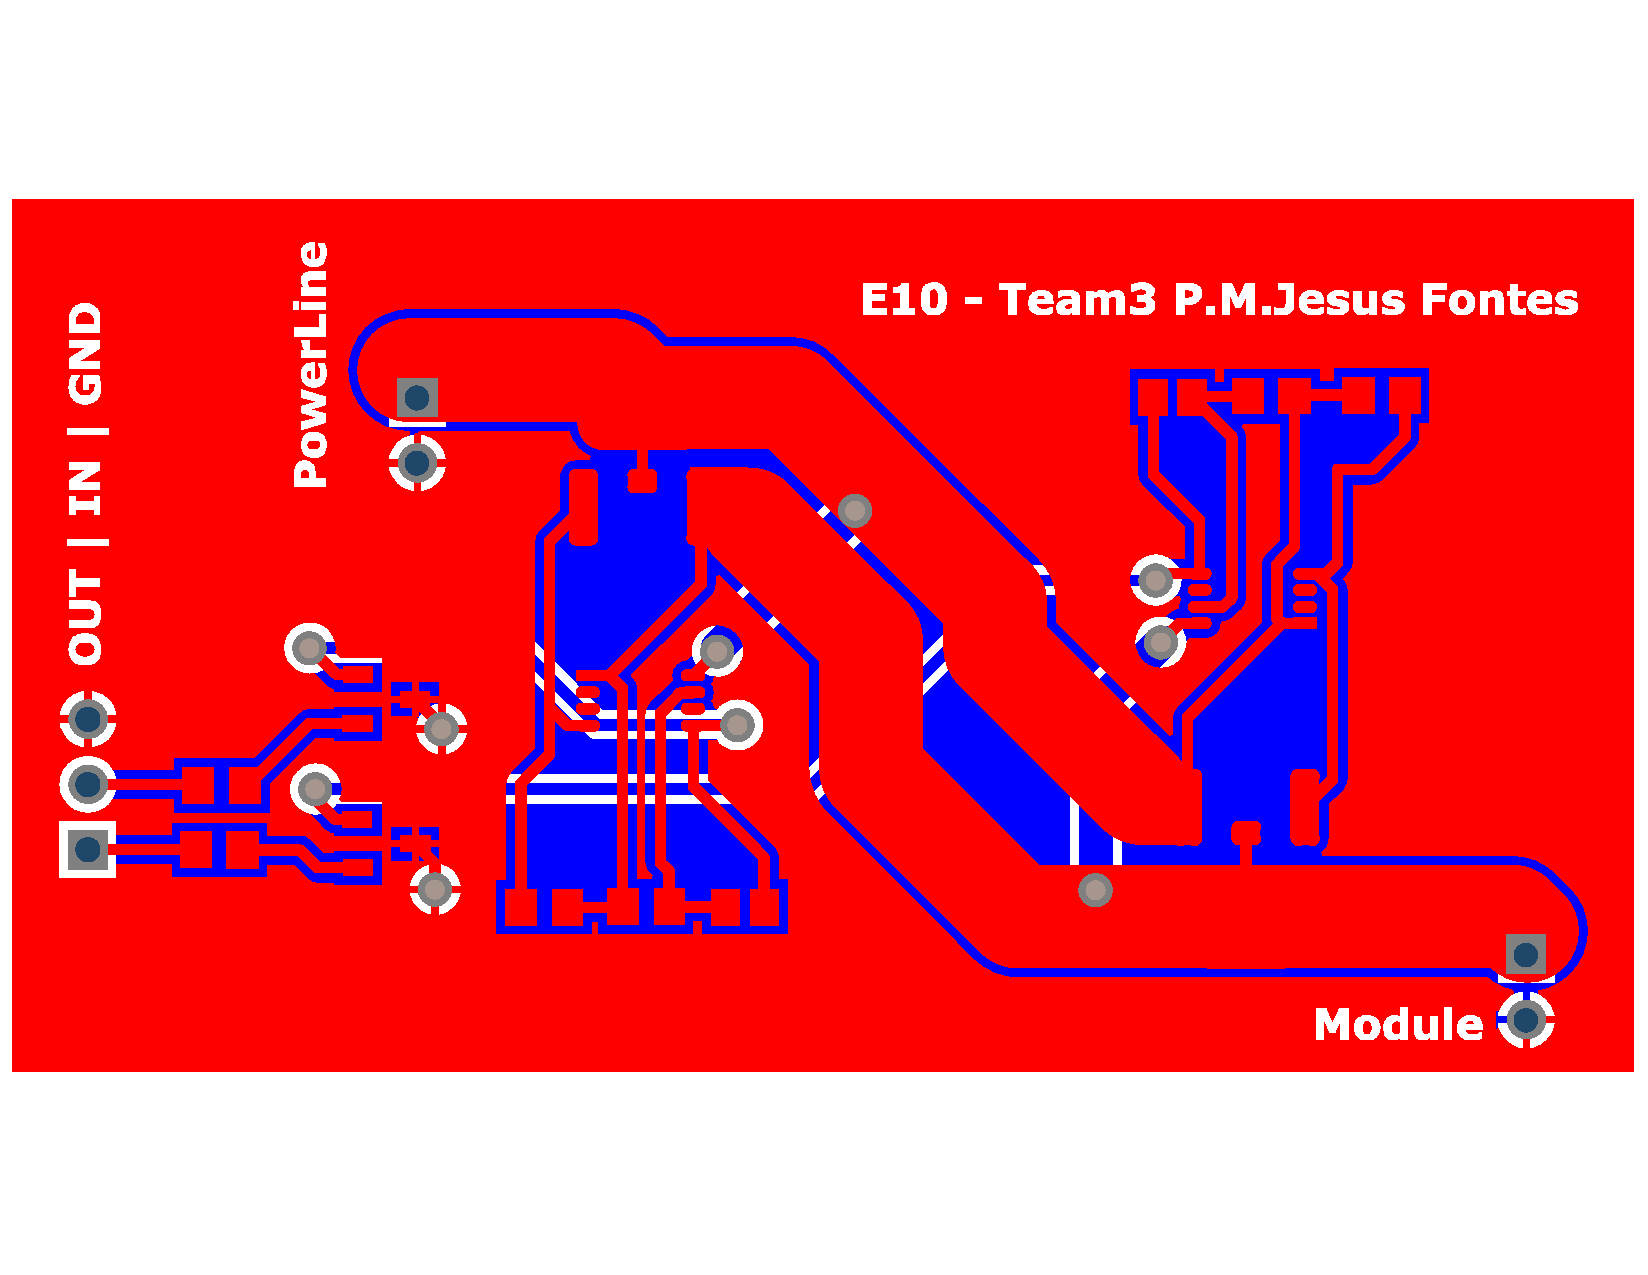
\includegraphics[width=0.7\textwidth,page=1]{images/ps_layout.pdf}
		\caption{PCB layout}
	\end{centering}
\end{figure}

\subsubsection{Mount component}

\begin{figure}[H]
	\begin{centering}
		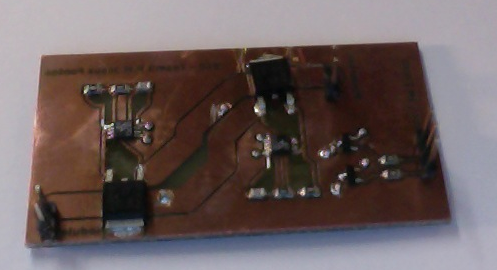
\includegraphics[width=0.6\textwidth,page=1]{images/mounted.png}
		\caption{Mounted PCB}
		%\missingfigure{Photo of the PS device}
	\end{centering}
\end{figure}

\subsubsection{Power Switch Test}
To test our circuit a load is applied on the module side and a source of 12V in the power-line connection. In a second scenario the opposite is done where a load is connected to the power-line and a source of 12V to the module side.
With this configuration is possible to test the current flow in both directions using the switch component of this circuit.
\paragraph{Test overview}
\textbf{Scenario 1:}
\begin{figure}[H]
	\begin{centering}
		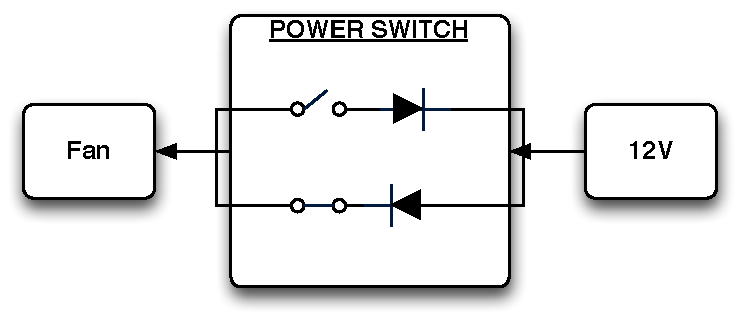
\includegraphics[width=0.6\textwidth,page=1]{images/scenario1.pdf}
		\caption{Current flow from the power-line to the module (fan)}
	\end{centering}
\end{figure}
\textbf{Scenario 2:}
\begin{figure}[H]
	\begin{centering}
		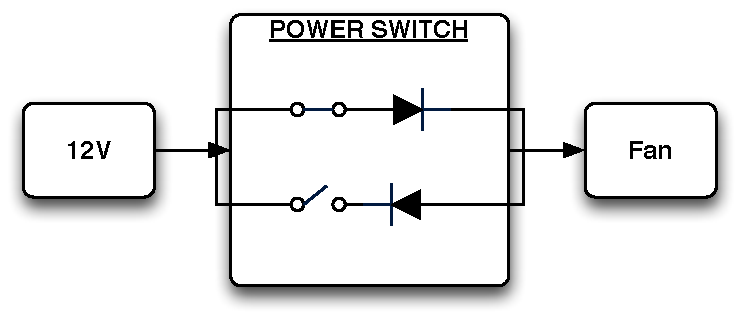
\includegraphics[width=0.6\textwidth,page=1]{images/scenario2.pdf}
		\caption{Current flow from the module to the power-line (fan)}
	\end{centering}
\end{figure}
\subsubsection{Further Implementation}
\begin{itemize}
	\item The power switch module does not work as expected, unfortunately current is also flowing in the opposite direction. Further tests have to be done in order to find a solution for this situation.
	\item A current sensor have to be add to each switching port ( 10 ports ), to surveillance the connected modules and react if a high\//low current is measured. From the measurements it is also possible to verify the efficiency of the green system.
	\item The module will connect to a main board with a card edge connection, so it will be easier to substitute in case of a malfunction and keep the housing free of many wires.
\end{itemize}


\subsection{Webserver Communication}

\subsubsection{Data Flow}
In the implementation of this system the user is able in an interactive way to command the power-switch. With this example is possible to send any command to the uClinux distribution running on the ARM7.
A webpage has been made with 4 check lists, each one corresponding to each LED on the board,  on click the LEDs are switched on and off.
\begin{figure}[H]
	\begin{centering}
		 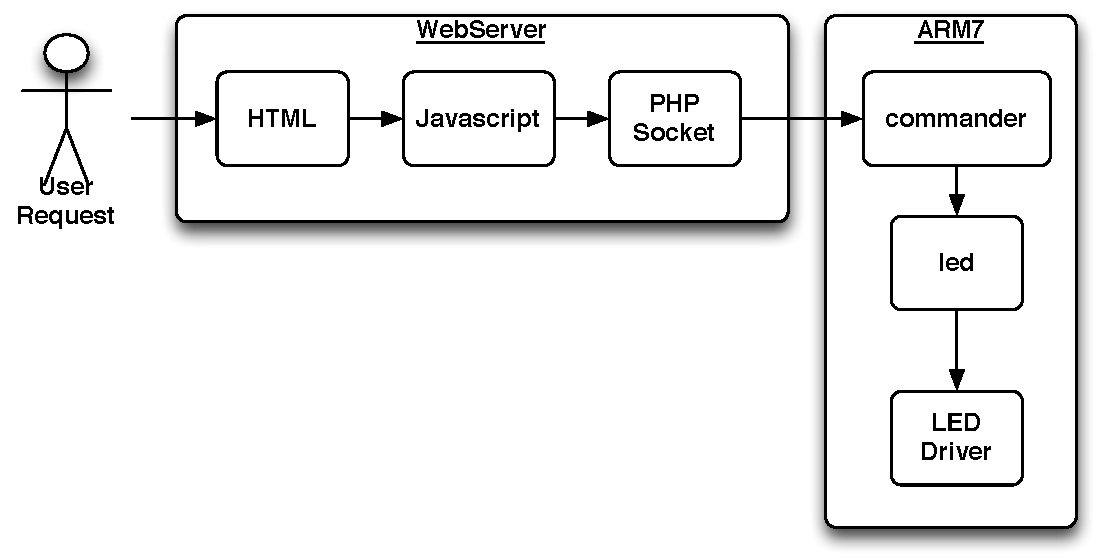
\includegraphics[width=1.0\textwidth,page=1]{images/dataflowPHP.pdf}
		\caption{Data Flow between user and ARM 7}
	\end{centering}
\end{figure}

\subsubsection{Setting the Server}
The server was set on the development environment and can be access at 10.1.18.223, no online status is given from the board. This webpage is used as verification of the development process with a low level interaction. 
\begin{figure}[H]
	\begin{centering}
		 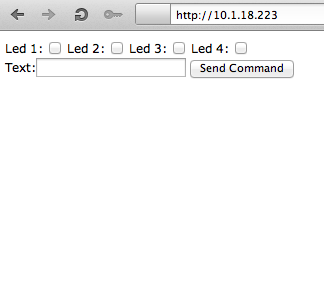
\includegraphics[width=0.4\textwidth,page=1]{images/website.png}
		\caption{Low level web interface}
	\end{centering}
\end{figure}

The PHP code creates a socket and connects to the ARM7 commander application, a TCP server listening to port 5555. The command is send to this application and then send to the shell, executing the application led from embedded artists:

Connection: connect.php

\begin{lstlisting}[language=php]
<?php
	
	function con(){
	
		require_once("globals.php");
		
		if ($_SESSION['socket']=socket_create(AF_INET, SOCK_STREAM, SOL_TCP)){
			echo "Socket created <br>";
		}
	
		if (socket_connect($_SESSION['socket'],$device_ip,$device_port)){
			echo "Connection stablished<br>";	
		} else {
			exit (socket_strerror(socket_last_error()));
		}
		echo socket_read($socket,1024)."<br>";	
	}    
?>
\end{lstlisting}

Command Handler: cmd.php

\begin{lstlisting}[language=php]
<?php
	
	session_start();
	
	include("connect.php");
	
	con();
		
	//Construct command
	$str = $_POST["cmd"];
	
	socket_write($_SESSION['socket'],$str);
	
	echo socket_read($_SESSION['socket'],1024);
	
	socket_close($_SESSION['socket']);
	
	$_SESSION["alive"]=false;

?>
\end{lstlisting}

Global Setting such as device IP and Port, the device IP in further implementation will be stored in the MYSQL database since the DHCP is activated on the board so we can have connection to the board even when a dynamic ip address is given.

globals.php

\begin{lstlisting}[language=php]
<?php
	
	//$device_ip = "127.0.0.1";
	$device_ip = "10.42.26.130";
	$device_port = 5555;
	
?>
\end{lstlisting}

The use of AJAX(Asynchronous Javascript And XML), allows the interface to be more dynamic and don't have to reload each time some action is taken, this is made in background by the XMLHttpRequest(). The code can be seen bellow, this use the method post to send variables and values.

\begin{lstlisting}[language=c]
function sendRequest(str){
	var req;
	if(window.XMLHttpRequest){
		req	= new XMLHttpRequest();
	} else {
		req = ActiveXObject("Microsoft.XMLHTTP");	
	}

	req.open("POST","cmd.php",false);
	req.setRequestHeader("Content-type","application/x-www-form-urlencoded");
	
	req.send("cmd="+str);
	alert(req.responseText);

}
\end{lstlisting}

\subsection{Further Implementations}
\begin{itemize}
	\item Implement the user interface generated in the Interactive Design sessions.
	\item Both direction communication is to be implemented, so the data can be retrieved from the board to the user.
	\item Website is active only when the board is on-line, otherwise the interface is inactive and a warning is sent to administrator.
\end{itemize}

\subsection{Device driver skeleton - Dennis}
The goal is to create a simple framework for creating device drivers for the LPC2478 platform. To do so, the scull example provided is used together with sample code provided with the uClinux distribution. The framework is tested by converting an ADC driver (running on the bare metal) into a device driver. Down below code snippets from the ADC is extracted an commented. 
\p The module registration is found in the \textit{file\_operations} structure:
\begin{lstlisting}[language=c]
static struct file_operations adc_fops = {
  .owner   = THIS_MODULE,
  .read    = adc_read,
  .open    = adc_open,
  //.write   = none,
  .release = adc_close,
};
\end{lstlisting}

The structure contains pointer values to the given functions, where these functions can be accessed from user space by:
\begin{table}[H]
	\centering
	\begin{tabular}{|l|l|l|}
		\hline
			Events		& User Functions & Kernel Functions \\ \hline
			Load Module 	& insmod	& module\_init()		 \\ 
			Open		& fopen	& file\_operations: open	 \\ 
			Read		& fread	& file\_operations: read	 \\ 
			Write			& fwrite 	& file\_operations: write	 \\ 
			Close		& fclose 	& file\_operations: release\\ 
			Remove		& rmmod 	& module\_exit()		 \\
		\hline
	\end{tabular}
	\caption{Function event table.}
\end{table}
Loading and removing a module is not included in the file operation structure, but declared aside as pointers to the two functions used:
\begin{lstlisting}[language=c]
// Define init and exit functions
module_init(adc_mod_init);
module_exit(adc_mod_exit);
\end{lstlisting}

In the init function several different things are done:
\begin{itemize}
	\item Setting up the registers (copy from the \textit{bare metal} driver file).
	\item Registration of the device (no need for dynamic numbering, so the major number is a static number not used by other drivers.)
	\item Allocating the char driver and adding it to the environment.
\end{itemize}

Code pieces from setting up the ADC:

\begin{lstlisting}[language=c]
//Register the device
	dev = MKDEV(adc_major, adc_minor);
	result = register_chrdev_region(dev, NUM_ADC_DEVICES, "adc");
//Allocate and add the adc device.
	adc_cdev = cdev_alloc();
	cdev_init(adc_cdev, &adc_fops);
	adc_cdev->owner = THIS_MODULE;
	adc_cdev->ops   = &adc_fops;

	result = cdev_add(adc_cdev, dev, NUM_ADC_DEVICES);
	
static void adcInit(void){
	volatile u32 tmp = 0;
	m_reg_bfs(PCONP, (1 << 12)); //Power on ADC
	m_reg_write(AD0CR, 0);
	m_reg_write(AD0CR,
			(4<<8)			|	//set clock division factor
			(0<<17)			|	//CLKS  = 0, 11 clocks = 10-bit result
			(1<<21)			|	//PDN   = 1, ADC is active
			(1<<24));			//start a conversion
	}
\end{lstlisting}
The exit function undoes the steps done in the initialization function.
\p Before reading the ADC channels, the channel shall be opened for reading. In the ADC code the pins are setup to be of type ADC. As the pins belongs to different PINSEL registers, a if else statement is used to set the right registers.
\begin{lstlisting}[language=c]
// inside the function: 
static int adc_open(struct inode* inode,  struct file* file){

// Check if the channel has been verified
if(chRefCnt[channel] == 0){
	file->private_data = (void *) channel;
	if(channel >= 0 && channel <=3)
		m_reg_bfs(PINSEL1, enable_bits[channel]);
	else if(channel > 3 && channel < 6)
		m_reg_bfs(PINSEL3, enable_bits[channel]);
	else if(channel >= 6 && channel < 8)
		m_reg_bfs(PINSEL0, enable_bits[channel]);
}
chRefCnt[channel]++;
\end{lstlisting}
When finish reading, the file is closed again and the opposite operation is performed (deselect the ADC function for the proper IO pin).
\p When reading the ADC, the result retrieved is converted from decimal into a string before it is returned to the user. Reading and writing to and from the CPU registers is done through the kernel space functions \textit{m\_reg\_read} and \textit{m\_reg\_write}. So the register writes and reads in the driver file for the ADC is performed as parameters sent to these functions:
\begin{lstlisting}[language=c]
//start conversion now (for selected channel)
m_reg_write(AD0CR, ((1 << channel) | (1 << 24)));

//wait til done
while ((m_reg_read(AD0GDR) & (1<<31)) == 0);

//get result from global register and adjust to 10-bit integer
result = (m_reg_read(AD0GDR) >> 6) & 0x3FF;
\end{lstlisting}

\subsubsection{Testing the driver - Dennis \& Paulo}
To proper test the driver, a small user space program has been written. The program opens the device, reads it and closes it again.
The argument sent to the program selects which channel should be read (ad0, ad1, ad2 etc.).

\begin{lstlisting}[language=c]
#define ADC "/dev/adc"
	
	//Format string to "Analog value"
	//Ex 1023 -> 3.30
void stringFormat(int value){
	char str[10];
	if((value%100)>9)
		sprintf(str, "%i.%i",value/100,value%100);
 	else
 		sprintf(str, "%i.0%i",value/100,value%100);
 		
	printf("%s\n",str);
}

int main(int argc, char *argv[]) {
	FILE *fp;
	char read[10];

	if ((fp = fopen(strcat(ADC,argv[1]),"r"))==NULL){
		printf("Cannot open file.\n");
		exit(0);
	}
	
	fread(read,1,10,fp);
	stringFormat(atoi(read)*330/1023);
	fclose(fp);
	return 0;
}
\end{lstlisting}

The application is compiled with the uClinux image using the tutorial at Klaus Kolles wiki\footnote{\url{http://klaus.ede.hih.au.dk/index.php/How-to_add_a_user_space_application_to_uClinux}}

\subsection{Host controller - Theis}
The host controller takes commands from the ARM7, and controlling blocks in the Spartan6. This controller is made in hardware and implemented in the Spartan6.
\begin{figure}[H]
	\begin{centering}
		 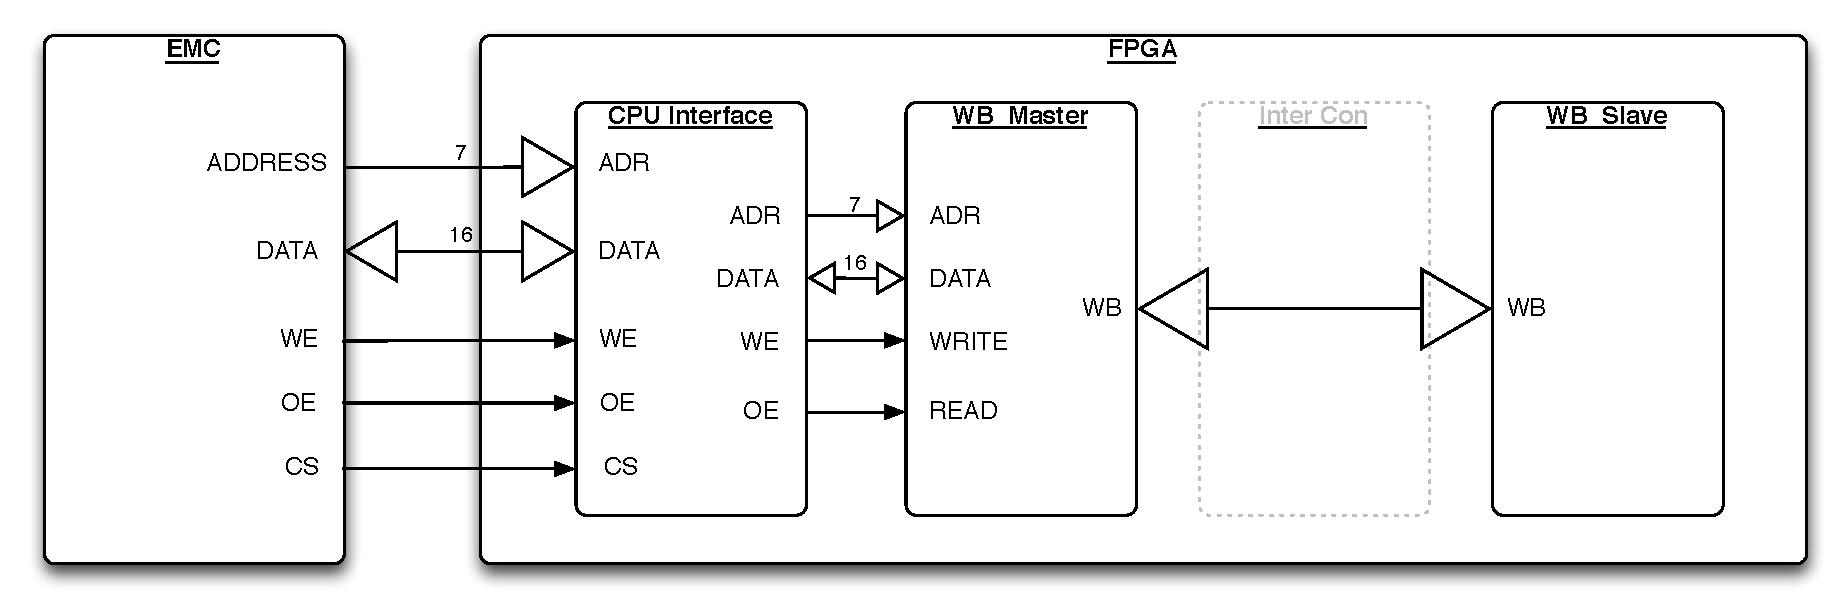
\includegraphics[width=1.0\textwidth]{images/host_controller.pdf}
		\caption{Host controller}
		%\missingfigure{host controller diagram}
	\end{centering}
\end{figure}
\subsubsection{External memory controller}
The EMC is a memory controller peripheral that support asynchronous static memory device such as RAM, ROM and flash. The chip select is used to select which memory device the ARM7 wants to communicate with. A block diagram of the EMC is shown below.
\begin{figure}[H]
	\begin{centering}
		 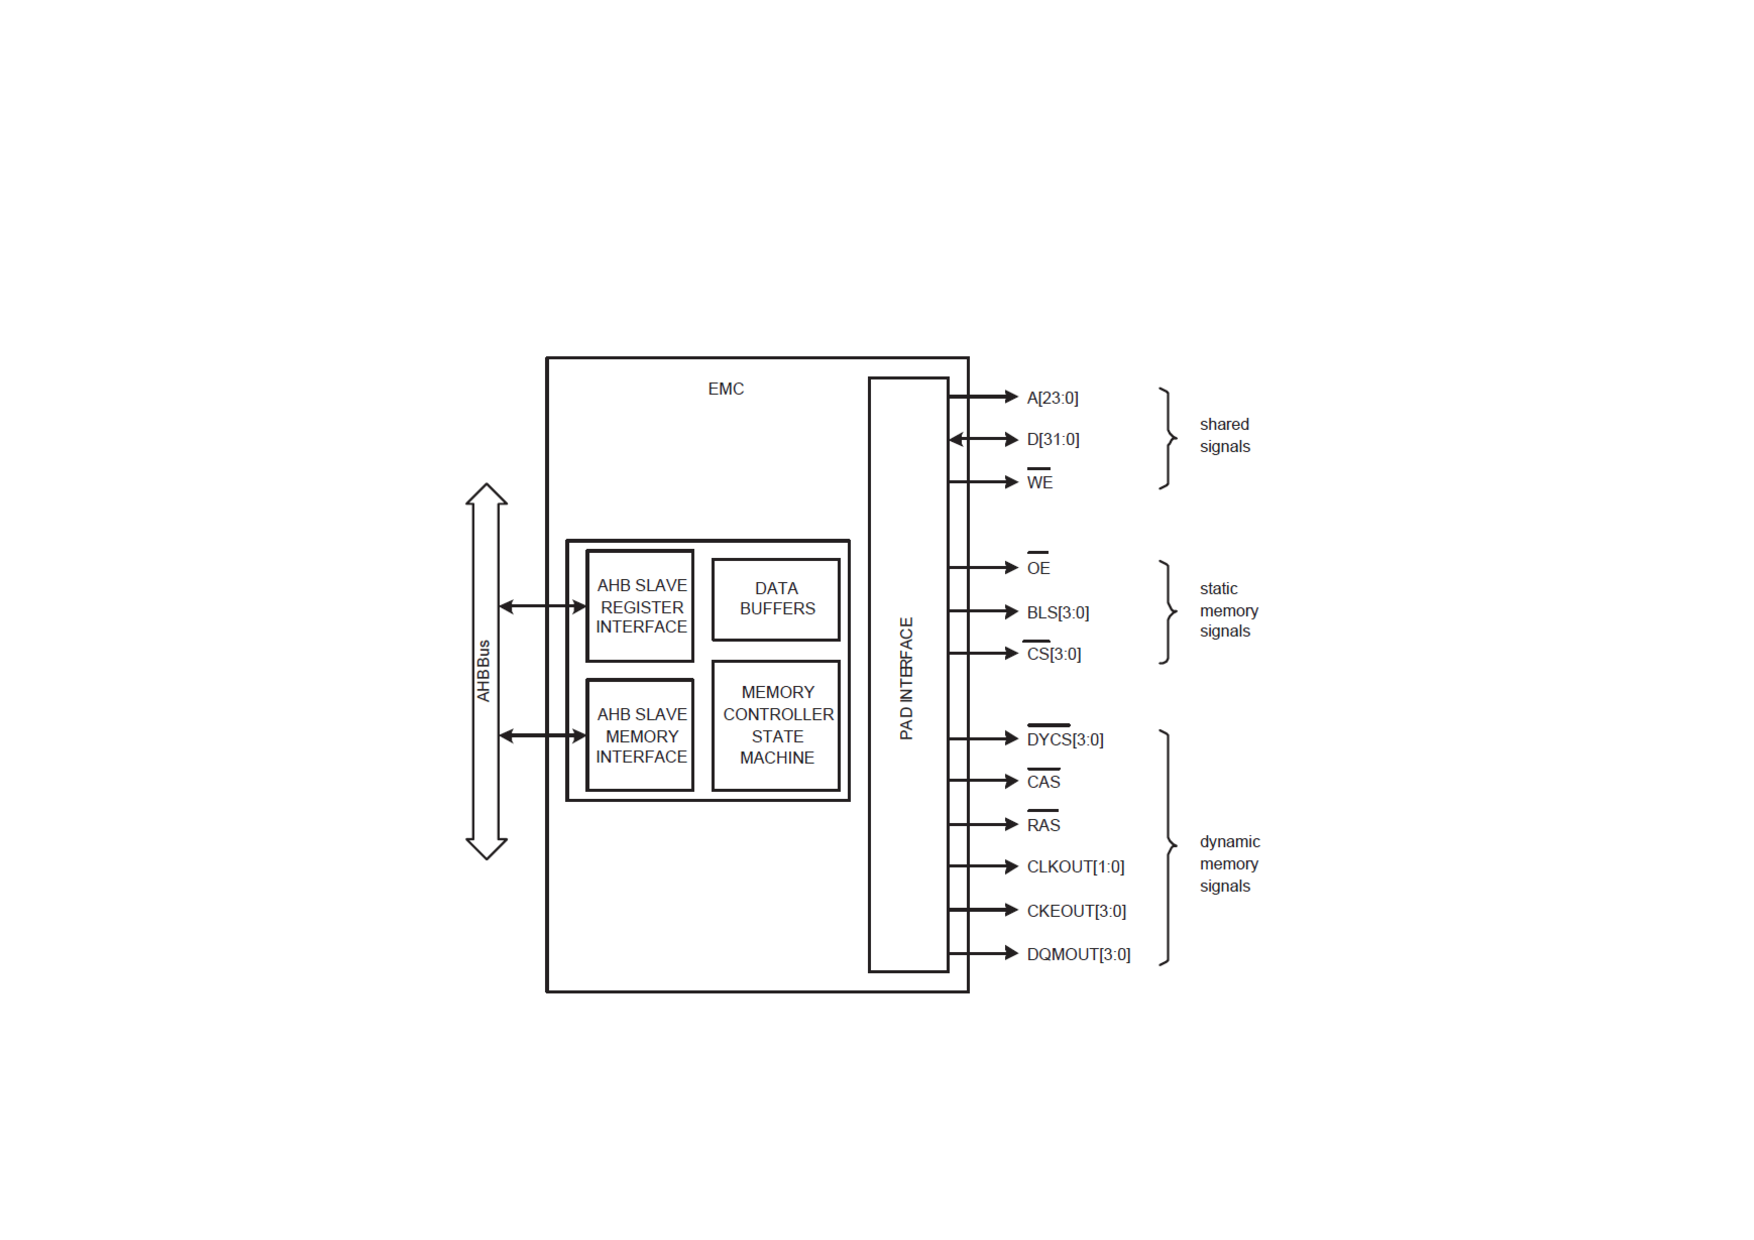
\includegraphics[width=0.7\textwidth]{images/emb_block_diagram.pdf}
		\caption{EMC block diagram}
		%\missingfigure{host controller diagram}
	\end{centering}
\end{figure}
The EMC is used to communicate with the Spartan6 board, with a 7 bit address and a 16 bit data bus, plus a read, write and chip select signal to indicate if it wants to read or write data, and select that it is the Spartan6 it would like data from. In this project the EMC is only used in static mode without the byte lane selects. A diagram of the EMC block is shown below.
\subsubsection{CPU interface}
The CPU interface communicate with the EMC on one site and with the master wishbone on the other site. The purpose of this interface is to determine if the EMC wants to communicate with the Spartan6, and if the ARM7 wants to read or write data.

\begin{lstlisting}[language=VHDL]
process (Clk,Rst)
	begin  
		if Rst = '1' then								--Reset set everything to 0
			Wr_o	<= '0';
			Rd_o	<= '0';
			A_o		<= (others => '0');
			D_o		<= (others => '0');
			CpuD_o	<= (others => '0');
		elsif (Clk'event and Clk = '1') then
			if CpuCs_i = '1' then					--Check chip select
				A_o	<= CpuA_i;							--Adress routing
					if CpuRd_i = '1' then			--Reading
						Rd_o	<= CpuRd_i;
						Wr_o	<= CpuWr_i;
						CpuD_o	<= D_i;					--Wishbone data out to Cpu data input
					elsif CpuWr_i = '1' then	--Writing
						Wr_o	<= CpuWr_i;					
						Rd_o	<= CpuRd_i;
						D_o		<= CpuD_i;				--Cpu data output to wishbone data input
					else
						Wr_o	<= CpuWr_i;		
						Rd_o	<= CpuRd_i;
						D_o		<= CpuD_i;
						CpuD_o	<= (others => '0');
					end if;
			else													--If chip select not high everything is set to 0
				Wr_o	<= '0';	
				Rd_o	<= '0';
				D_o		<= (others => '0');
				A_o		<= (others => '0');
				CpuD_o	<= (others => '0');
			end if;
		end if;
end process;
\end{lstlisting}
The block is synchronous with the clock and have an asynchronous reset. If the reset is pressed everything is set to zero to tell the master wishbone to not do anything. When the chip select is high, it tells the block that the ARM7 want to communicate with the Spartan6. After chip select is activated, the block checks if the ARM7 want to read or write data from or to the Spartan6. If the ARM7 wants to read data, the interface block routes the data from master wishbone to the data vector on the EMC. Otherwise if the ARM7 wants to write data, the data vector on the EMC is routed to the data input for the master wishbone. In any case of read or write the read and write output from the EMC is routed to the master wishbone. The address input from the EMC is routed as soon as the chip select is activated. If the chip select is not active, everything is set to zero, to secure that the master wishbone do not write any data. The data output to the EMC is tri-stated in the wrapper code if the chip select is not active, to not disturb other communication on the EMC bus.
\paragraph{Test bench}
The test bench is made to test if the host controller is responding correct to different signals, image of the test bench signals is shown below.
\begin{figure}[H]
	\begin{centering}
		 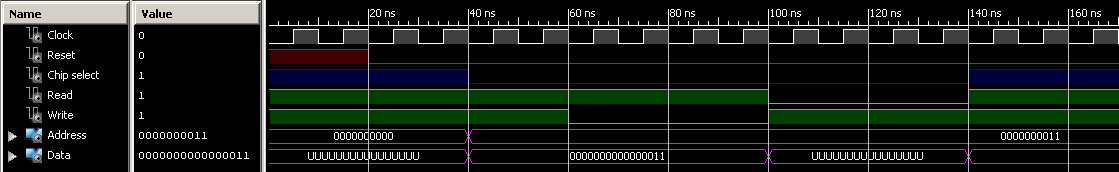
\includegraphics[width=1.0\textwidth]{images/host_controller_tb.png}
		\caption{Host controller test bench}
		%\missingfigure{host controller diagram}
	\end{centering}
\end{figure}
The test bench shows that after the reset state and when the chip select is active, a write cycle is made,to address "0x03" and the data that is written is "0x03". After the write, a read cycle on address "0x03" and the data read is uninitialized, this is because the master wishbone do not get any data from slave, so it is not possible to send any valid data to the ARM7, so the uninitialized indicate so far that the read cycle works. And after the chip select deactivate the data is equal to the data from the ARM7.
\subsubsection{Wishbone}
Wishbone is a computer bus for integrated circuit communication. It sets up some standard communication rules to use when designing IP cores. This makes it easy to reuse code on different hardware and in different systems. The wishbone bus is a logic bus, this means that there is no rules for voltage levels, it only works with ones and zeros. In this project the wishbone is used as illustrated on the picture below.
\begin{figure}[H]
	\begin{centering}
		 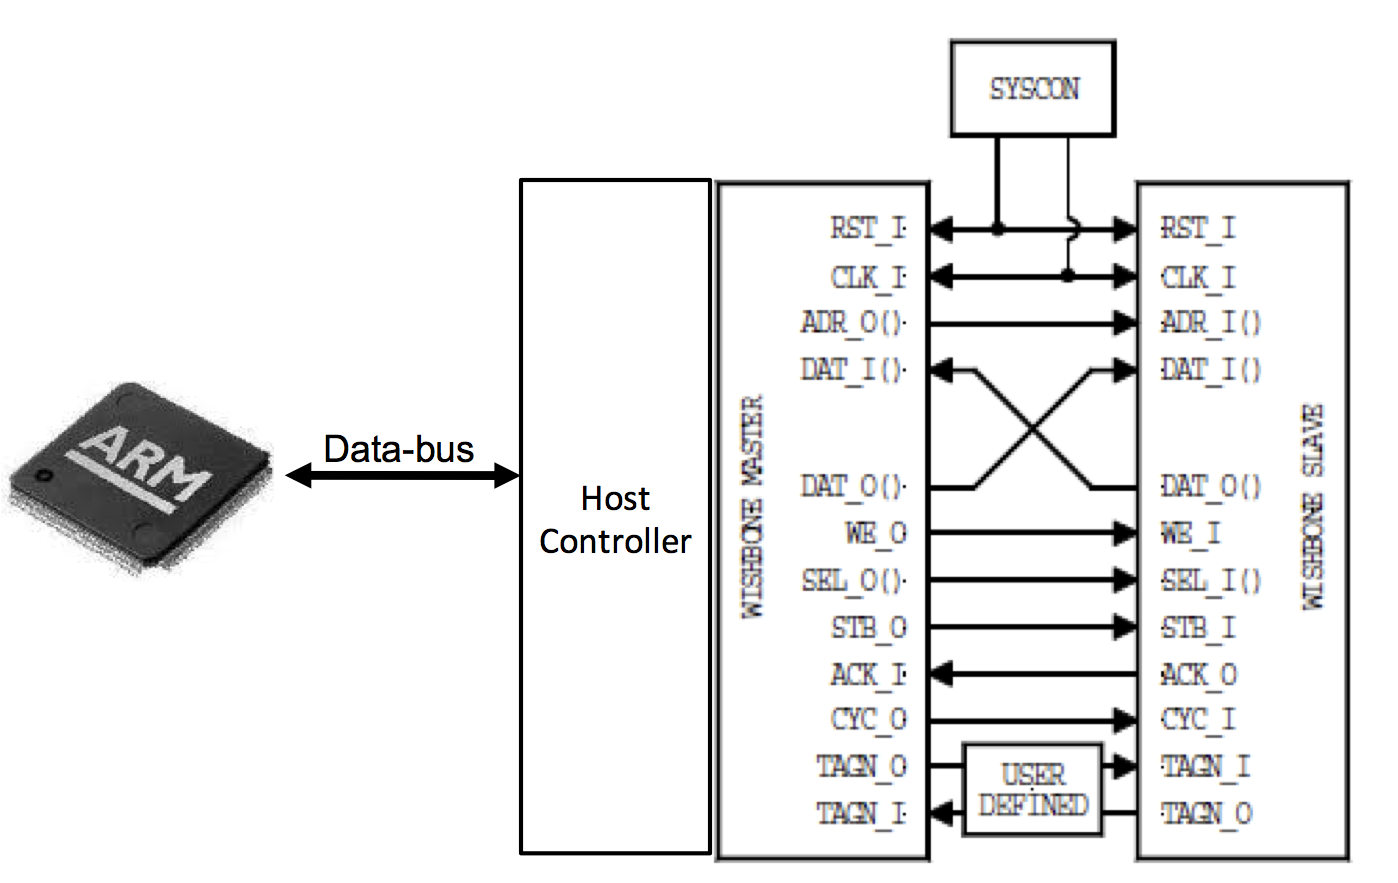
\includegraphics[width=0.8\textwidth]{images/typical_usage.png}
		\caption{Wishbone connection for the host controller}
		%\missingfigure{host controller diagram}
	\end{centering}
\end{figure}
The EMC on the ARM7 is controlling the wishbone master, which is controlling all the wishbone slaves that is in the system. This make it easier to write a driver for the ARM7 that controls the master wishbone through the EMC. Then the master wishbone control every IP core with at wishbone slave interface connected. In this project the wishbone is going to use single read and write cycles, the single read cycle timing diagram is shown below.
\begin{figure}[H]
	\begin{centering}
		 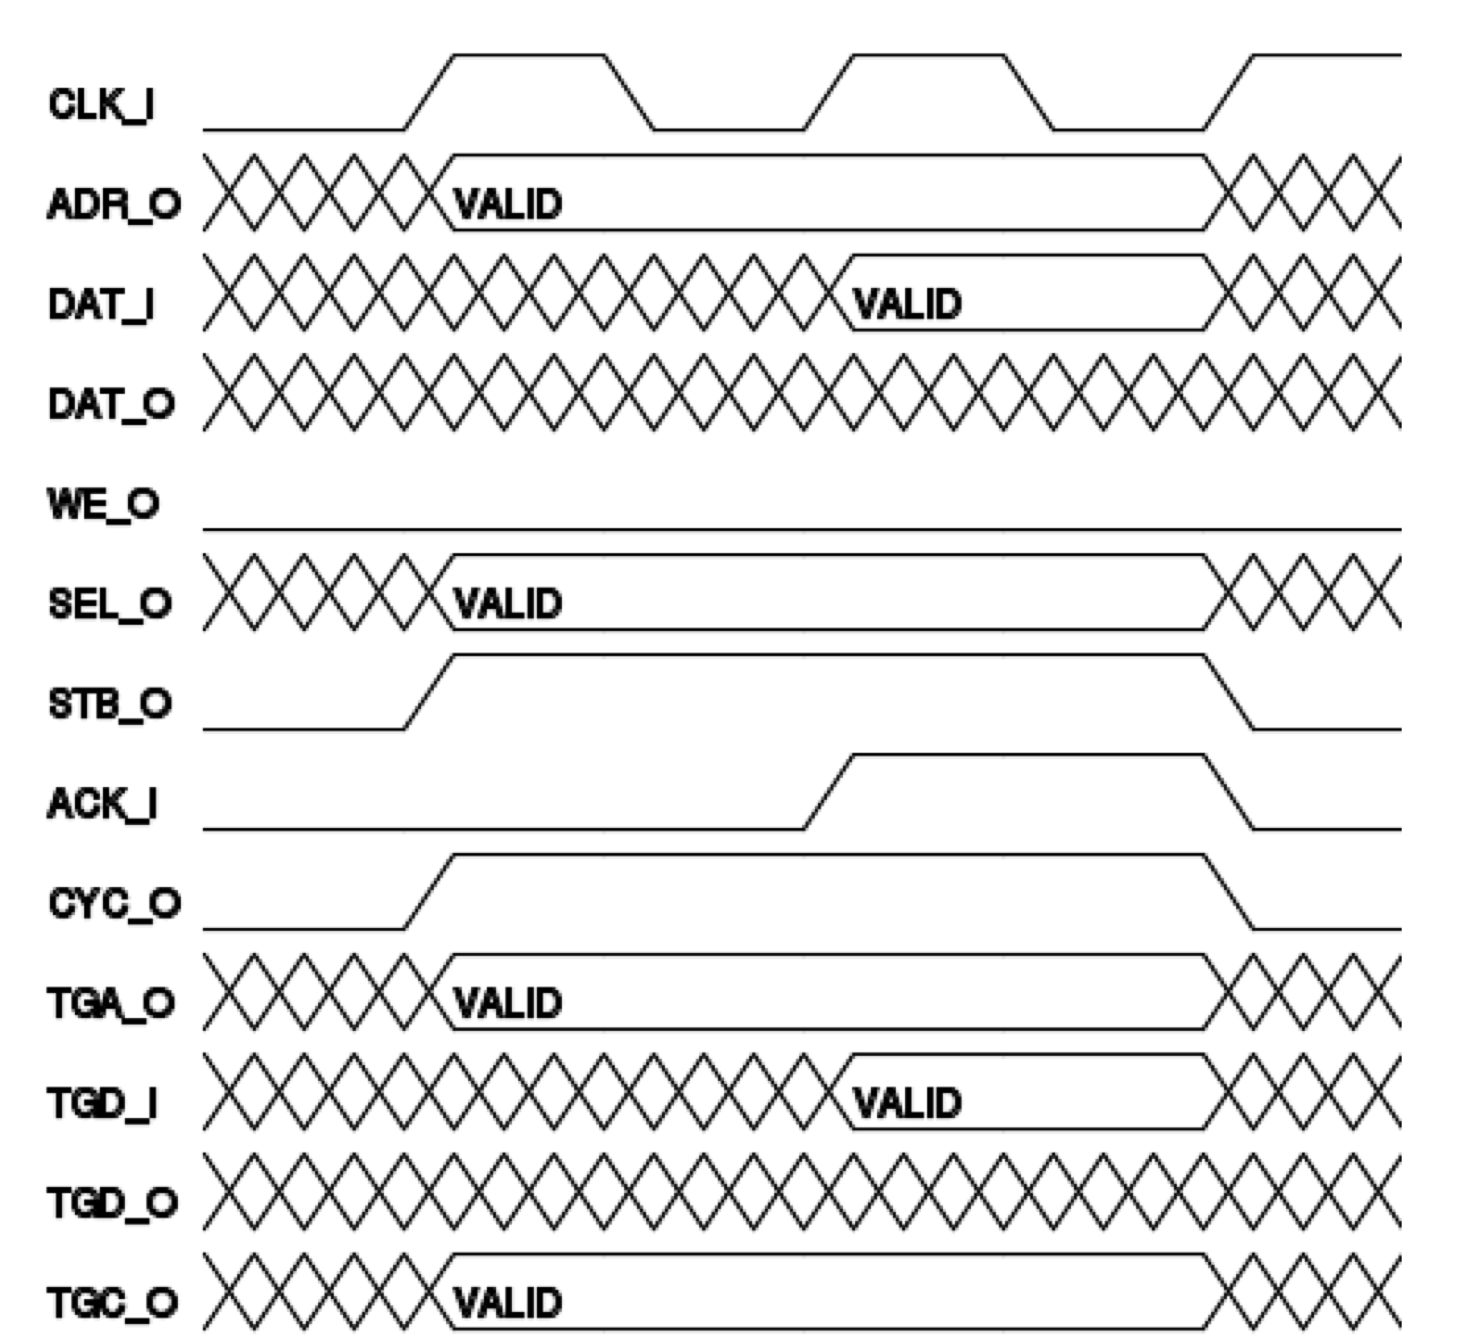
\includegraphics[width=0.65\textwidth]{images/wb_single_read.png}
		\caption{Single read cycle}
		%\missingfigure{host controller diagram}
	\end{centering}
\end{figure}
When a single read cycle is started, the master wishbone presents a valid address, on the address register, it sets the write enable to zero to show that this is a read cycle, the SEL\_O is set, to show where on the data input it expect the data to be read, it also sets the CYC\_O and STB\_O high to indicate the start of a cycle and a phase.

On the next raising clock edge, the slave decodes the input and sets the acknowledge bit high in response to the SEL\_O. It also presents valid data on the slave data output. The master monitors the acknowledge and prepares to latch data.


On the third raising clock edge the master wishbone latches the data, and set the STB\_O and CYC\_O to zero to end the cycle and the phase, the slave set the acknowledge bit low again as response to STB\_O.\\
The timing diagram for the single write cycle is shown below.
\begin{figure}[H]
	\begin{centering}
		 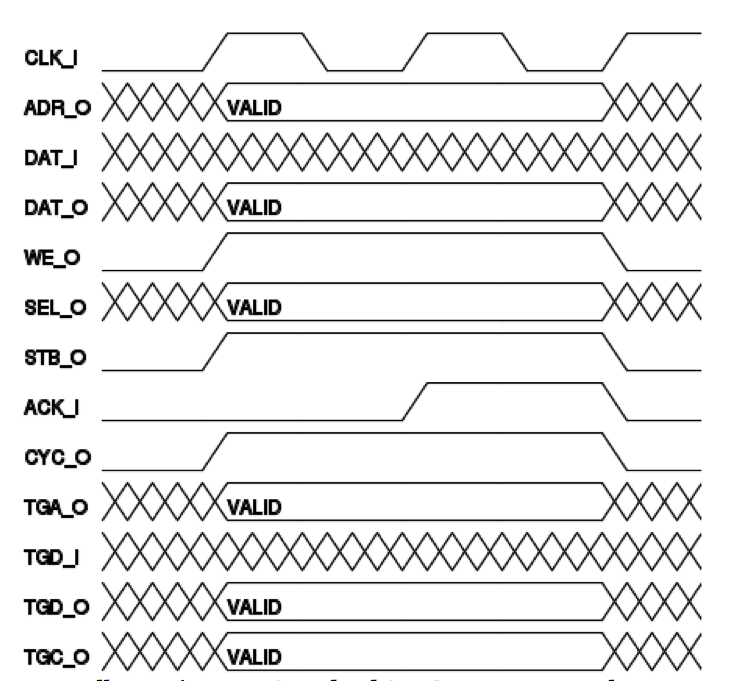
\includegraphics[width=0.65\textwidth]{images/wb_single_write.png}
		\caption{Single write cycle}
		%\missingfigure{host controller diagram}
	\end{centering}
\end{figure}
When the master wishbone wants to write to the slave, it present valid address and data on the address register and data output, it also sets the write enable high to indicate the cycle is write. As with the read the STB\_O and CYC\_O is set high to indicate cycle and phase start, all this is done on the first raising clock edge.

On the second raising clock edge the slave decode the input and set the acknowledge bit high in response to the SEL\_O. It also prepares to latch data from the master. The master monitors the acknowledge bit and prepare to terminate the cycle.

On the last raising clock edge the slave latches the data, the master set the STB\_O and CYC\_O to zero to end the cycle and the phase, the slave set the acknowledge bit low again as response to STB\_O.

\subsection{Post deployment}
Spend a short time evaluating the just-closed timebox. What went well? Why did it go well? What caused problems? Can they be prevented in the future? And how can they be prevented?
\subsubsection{Power switch}
\subsubsection{Host Controller}
The host controller work in theory but still needs to be tested in practice. The handed out code, was well commented to give a good overview. This made it easier to make the code for CPUinterface.
